\newpage
\section {Билет 13. Обработка текстов. Морфологический анализ, tf*idf, ранжирование, исправление опечаток, классификация, кластеризация, поиск дубликатов.}

Пусть у нас есть пачка текстов $T_1, T_2, T_3 \dots T_n$, которую мы будем исследовать. \\
Методы представления текстов:
\begin{itemize}
\item множественный. Текст представляется как множество слов, для которых не определено отношение порядка. Преимущество - простота. Для вычисления сходства двух текстов используется простая формула $k = \frac {|A \cup B|}{|A \cap B|}$. Если коэффициент большой, то тексты похожи друг на друга;
\item векторная модель. Пусть есть выделенные  "базисные" слова $w_1, w_2, \dots w_n$, тогда текст представляется вектором в n-мерном пространстве, где, в простейшем случае, координаты вектора строятся так: i - ая координата это количество вхождения слова $w_i$ в текст. Но на практике используют другой способ определения координат (способ с помощью модели tf*idf).
\end{itemize}

\subsubsection {Модель tf*idf для построения векторов}
\href{https://clck.ru/EqWAS}{Векторная модель} 
\begin{defn}
tf для слова $w_i$ в тексте $T_j$ определяется так: 
 $tf = log (Q)$, Q - сколько раз $w_i$ встретилось в $T_j$.  \\
idf для слова $w_i$ в тексте $T_j$ определяется так: 
$idf = \frac{1}{log(P)}$, P - количество документов в последовательности $T_1, T_2, T_3 \dots T_n$, в которых встречается слово $w_i$. 
\end{defn}
На практике используют именно произведение $tf*idf$ - означающее важность слова в документе. Произведение tf*idf отражает закон Зипфа:
На графике по вертикальной оси откладывается важность (т.е. tf*idf), а горизонтальной частота встречаемости слова в конкретном документе. 
Выделяется три зоны: \\
1 - редкие слова, слова придуманные автором или опечатки \\
2 - ключевые слова, определяющие текст \\
3 - обычные слова связки \\

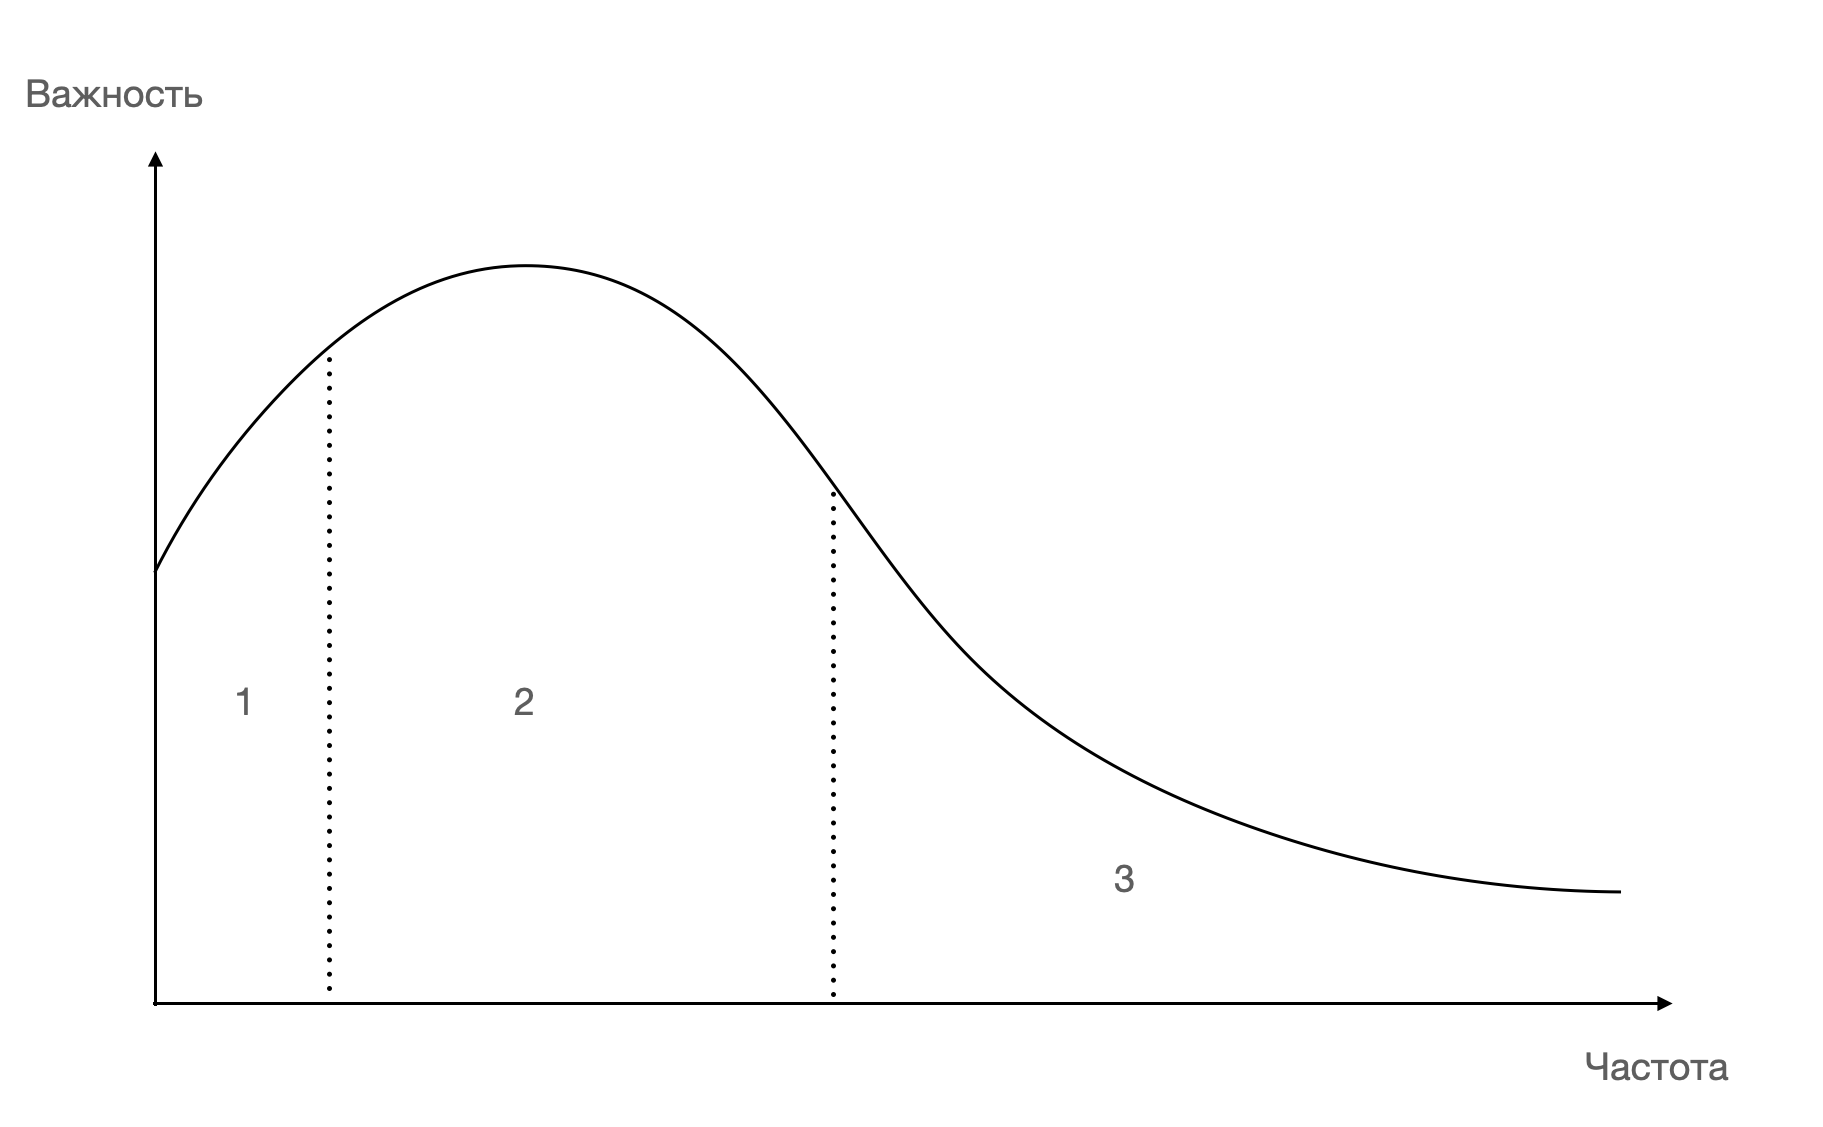
\includegraphics[width=0.5\linewidth]{13/Zipf}
Поэтому, в итоге, текст это вектор, где на i - ом месте стоит tf*idf слова $w_i$. Мера близости текстов A и B в векторной модели - косинус угла между векторами A и B.

\subsubsection {Морфологический анализ}
\href{http://prutzkow.com/ru-ru/science/natural-language-processing/morphology/}{Морфологический анализ} \\
Перед построением векторов сначала несколько унифицируют используемые слова, для этого используют морфологический анализ.
Морфологический анализ может быть словарным (со словарем основ и окончаний или словарем словоформ) или бессловарным (только со словарем окончаний; словарь окончаний может быть встроен в алгоритм морфологического анализа). Бессловарный метод используется только для определения переменной морфологической информации (не всегда однозначно), а словарный — во всех остальных случаях. 

\subsubsection {Исправление опечаток}
\href{https://clck.ru/A6RjQ}{Расстояние по Левенштейну} \\
Элементарная операция по Левенштейну - это добавление буквы, удаление буквы или замена одной буквы на другую. Расстояние это количество операций необходимое для того, чтобы из одного слова получить другое с помощью операций Левенштейна. Например, слова aabb, aabbb, aab, aacb находятся на одинаковом расстоянии (расстояние равно 1). Далее, чтобы исправить опечатку необходимо найти ближайшее слово по Левенштейну. Если использовать обычный линейный поиск, то процедура поиска может занять много времени. Поэтому используют поиск по дереву. В вершинах дерева расположены буквы, различные пути образуют слова. 

\subsubsection {Поиск дубликатов}
Если необходимо решить задачу на полное совпадение текстов, то она делается очень просто. Для каждого документа берется хэш-функция (например, MD5). С большой вероятностью документы с совпадающим значением хэш-функции совпадают. Но на практике необходимо искать не в точности совпадающие тексты, а просто похожие. В таком случае используют понятие N-грамм.  \\
\begin{defn} N-грамма — последовательность из подряд идущих N элементов. \end{defn}
Например для текста: Мама мыла раму, все 4 граммы имеют вид: мама, амам, мамы, амыл, мыла, ылар, лара, арам, раму.  \\
\begin{theorem}
Если документы почти совпадают, то и N-граммы почти совпадают.
\end{theorem}
Это отличный способ - сравнивать все N-граммы, но есть одна проблема - их очень много и сравнение всех N-грамм двух текстов займет много времени. Поэтому действуют следующим образом.

\begin {itemize}
\item Берутся все N-граммы двух текстов и к ним применяется какая-нибудь хеш-функция (Например, \href{https://clck.ru/9cRa4}{MD5}). (хэш-функция от N - граммы называется называется шинглом);
\item Береться 84 шингла (значения хэш-функции), они объединяются в 12 групп;
\item На каждой группе шинглов опять вычисляется хэш-функция. (значение хэш функции на группе шинглов называется супершинглом);
\item Если у двух текстов совпадает хотя бы один супершингл,  то они потенциально совпадают.
\end {itemize}

\subsubsection {Классификация и кластеризация}
Классификация - разделение текстов на группы, которые мы заранее определили. Кластеризация - разделение на группы, заранее неизвестные.
Примеры разделения: по авторству, по эмоциональной окраске текста, по цели (повествование/реклама), по различным темам.
Описанные ниже методы одинаково применяются для кластеризации и классификации.

\begin {itemize}
\item Тезаурус. Берется двудольный граф, в котором в одной доле (будем ее называть доля  W) располагаются термины, а во второй доле - темы (будем ее называть T). Вершина из W соединяется с вершиной из T, когда соответствующий термин описывает данную тему, на ребре соединяющем вершины приписывается число меньшее 1, показывающее степень соответствия термина теме (Например, термин "матрица" однозначно соответствует линейной алгебре, но может встречаться и в теории вероятностей (но встречается там гораздо реже, чем в линейной алгебре), тогда на ребре матрица-линейная алгебра будет, например, 0.7, а на ребре матрица-теория вероятностей -- 0.3 ). То есть в итоге имеем взвешенный двудольный граф. Данный граф дается нам лингвистами или формируется нами. Далее мы читаем полученный текст и если встречаем термин w из W, который соединен ребром веса p с темой t, то к теме t  прибавляем соответствующий вес p. Тема, у которой в результате чтения текста будет максимальное значение, тема текста. Минус этого метода: необходимо строить хороший двудольный граф, т.е. отвечающий современному состоянию языка;
\item Самообучающиеся карты.
Пусть стоит задача разделить цветные точки на группы так, чтобы в каждой группе были точки одного цвета. В начальный момент времени все точки расположены в трехмерном пространстве хаотично (Почему трехмерном? Каждый цвет однозначно представляется тремя числами в системе rgb (rgb - аддитивная цветовая модель, описывающая способ кодирования цвета для цветовоспроизведения с помощью трёх цветов, которые принято называть основными)). Выбираются функции $f_1, f_2, f_3$ как показано на рисунке (Функции определены на отрезке $[-3, 3]$ и интегралы $\int_{-3}^3 f_i (x) dx$ = 1 (На уровне идеи это требование означает, что цвет суммарно не меняется)).
Далее используется следующий алгоритм:
\begin {itemize}
\item Для точки A в ее окрестности считается сумма $S = \sum\limits_{p_i \in U} c (p_i) f_1 (\rho_i)$, где $U$ - окрестность точки A, $p_i$ - точки, принадлежащие этой окрестности, $c (p_i)$ - цвет точки $p_i$ (вектор в трехмерном пространстве), $\rho_i$ - расстояние от точки $p_i$ до точки A. Точка А красится в цвет S. Так последовательно делаем для всех точек. Может получиться так, что цвета $S$ не было среди цветов изначальных точек, но это нормально;
\item Проделываем процедуру еще раз с функциями $f_2, f_3$;
\item В итоге все точки разделятся на группы, причем, например, между синим и зеленым цветом будет желтый, а между синим и красным - фиолетовый.
\end {itemize}

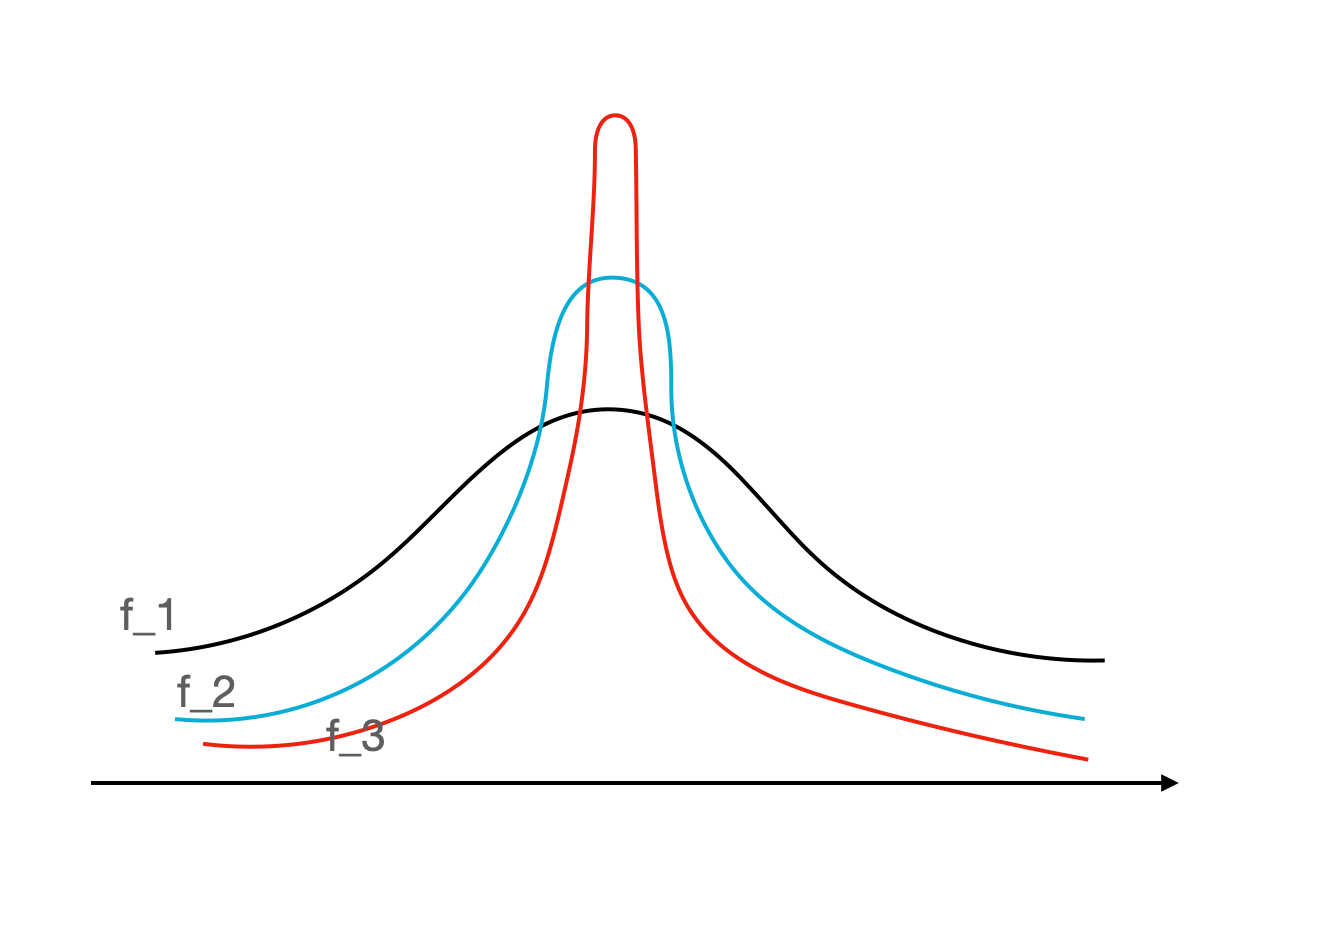
\includegraphics[width=0.5\linewidth]{13/func}

\begin{figure}[h!]
\begin{minipage}[h]{0.49\linewidth}
\center{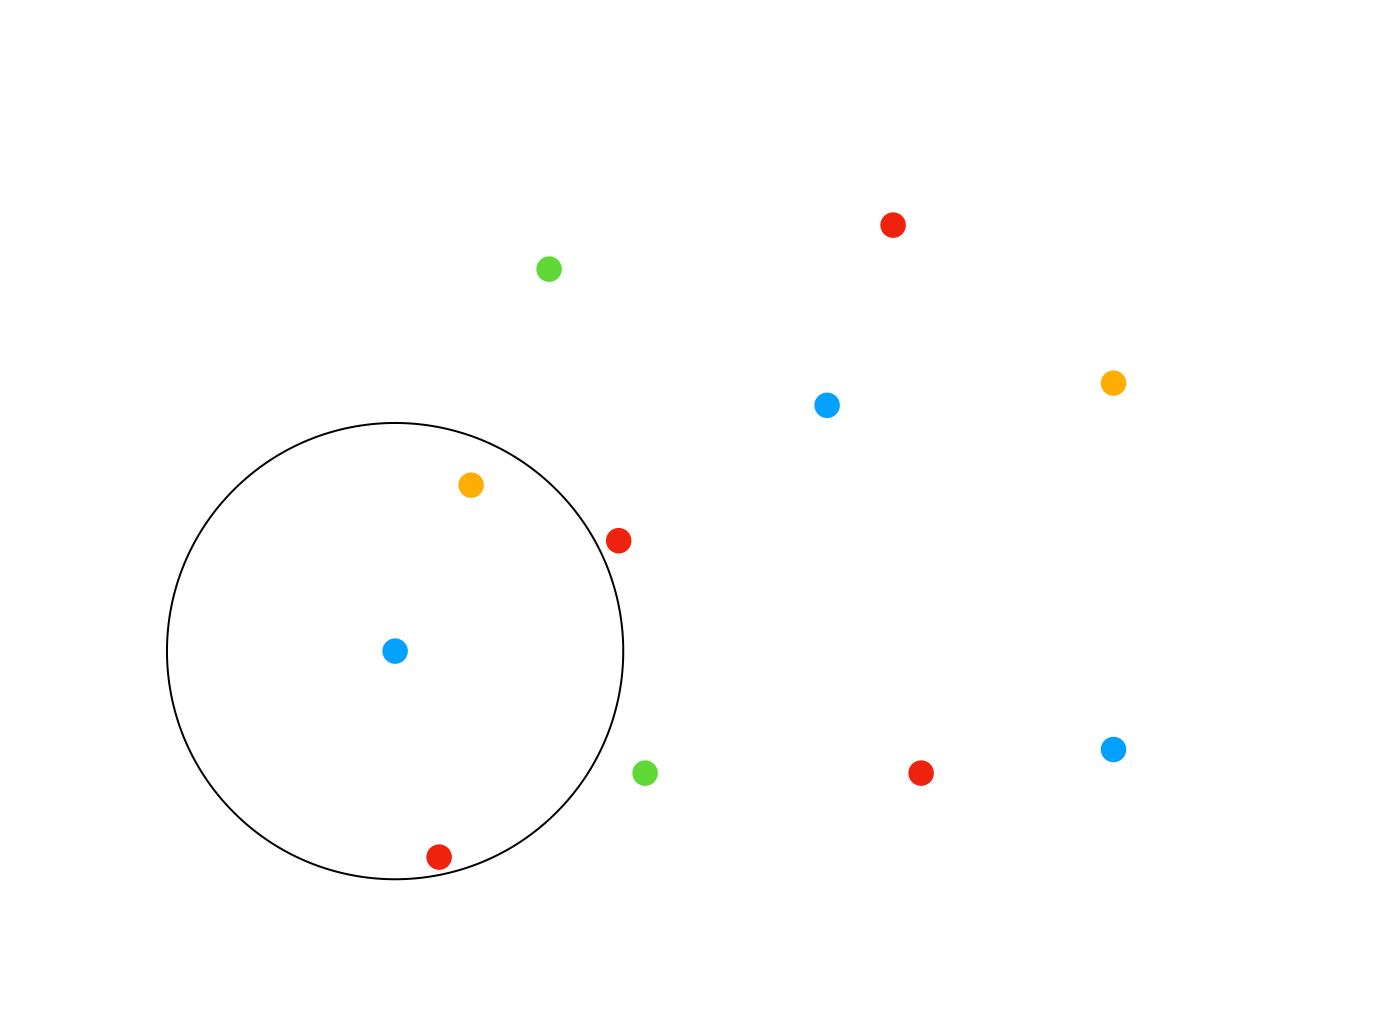
\includegraphics[width=\linewidth]{13/begin} положение точек до работы алгоритма \\}
\end{minipage}
\hfill
\begin{minipage}[h]{0.49\linewidth}
\center{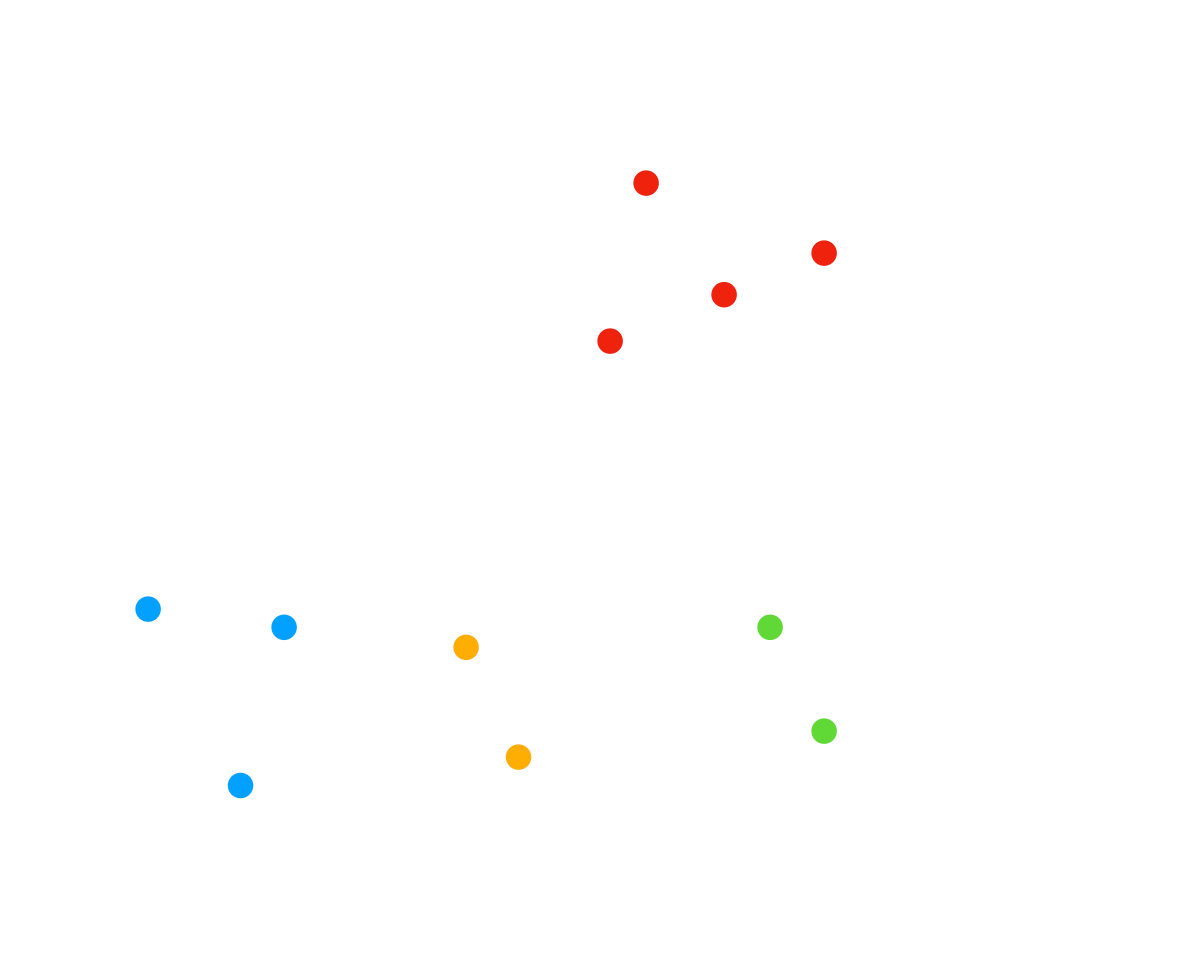
\includegraphics[width=\linewidth]{13/result} положение точек после работы алгоритма \\}
\end{minipage}
\end{figure}

\item  Физическая расстановка.
Стоит задача разделить точки на группы. Припишем каждой точке свою массу. Зададим векторы силы всемирного тяготения по формуле 
$\vec{F}_{A,B} = G \frac{m_{A} m_{B}\vec{r}}{|\vec{r}|^3}$, где $G$ - константа, $\vec{r}$ - вектор, соединяющий точки А и В, $m_{A} m_{B}$ - массы точек. Тогда за время $\Delta t$ каждая точка под действием равнодействующей силы притяжения передвинется на расстояние $\Delta s_i$ (свое для каждой точки). Если точки находятся близко, то объединяем их в одну точку суммарной массы. Алгоритм проводится до тех пор, пока нас не удовлетворит разделение на группы или точки не попадут в равновесное состояние.  

\item Геометрическая расстановка. (Наиболее часто встречаемый метод). Пусть есть точки на плоскости, которые мы хотим объединить в группы. (см. рисунки шаг 1-4)
\begin{itemize}
\item на шаге 1 имеем просто хаотично разбросанные точки;
\item на шаге 2 в произвольные места добавляем точки-кластеры, которые отвечают за образование групп;
\item на шаге 3 определяем какие точки к какому кластеру ближе;
\item на шаге 4 перемещаем кластеры в центр масс соответствующих точек и применяем шаг 3 к новой конфигурации;
\item шаг 4 продолжаем до тех пор пока кластеры не перестанут двигаться.
\end{itemize}

\begin{figure}[h]
\begin{minipage}[h]{0.47\linewidth}
\center{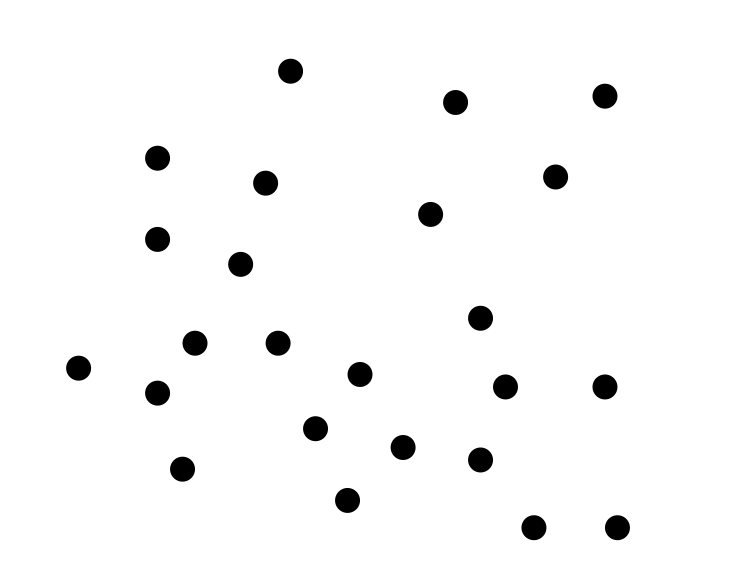
\includegraphics[width=1\linewidth]{13/1}}  \\ шаг 1
\end{minipage}
\hfill
\begin{minipage}[h]{0.47\linewidth}
\center{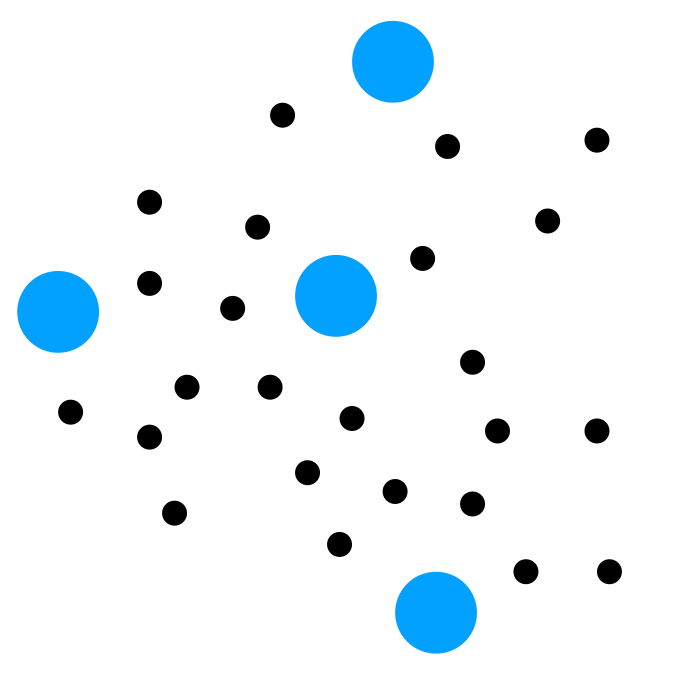
\includegraphics[width=1\linewidth]{13/2}} \\ шаг 2
\end{minipage}
\vfill
\begin{minipage}[h]{0.47\linewidth}
\center{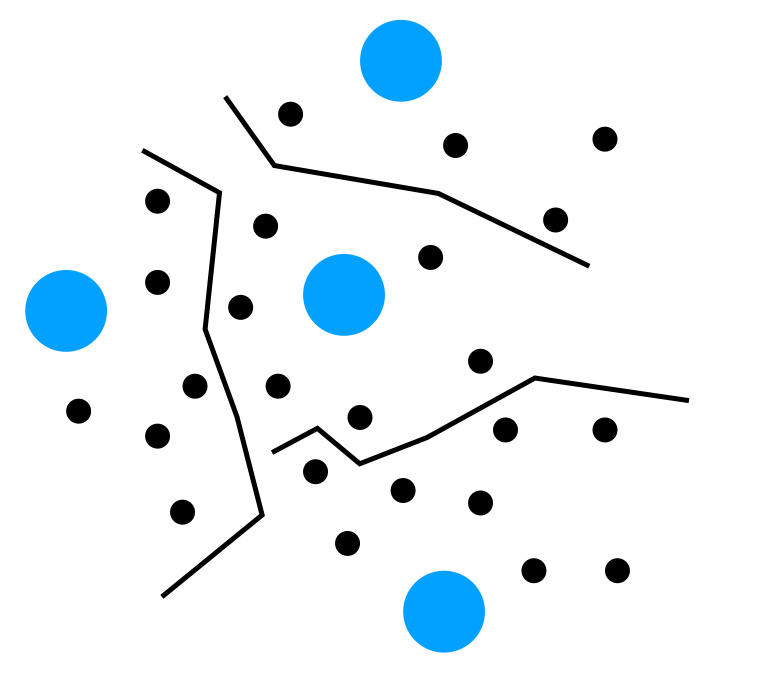
\includegraphics[width=1\linewidth]{13/3}} \\ шаг 3
\end{minipage}
\hfill
\begin{minipage}[h]{0.47\linewidth}
\center{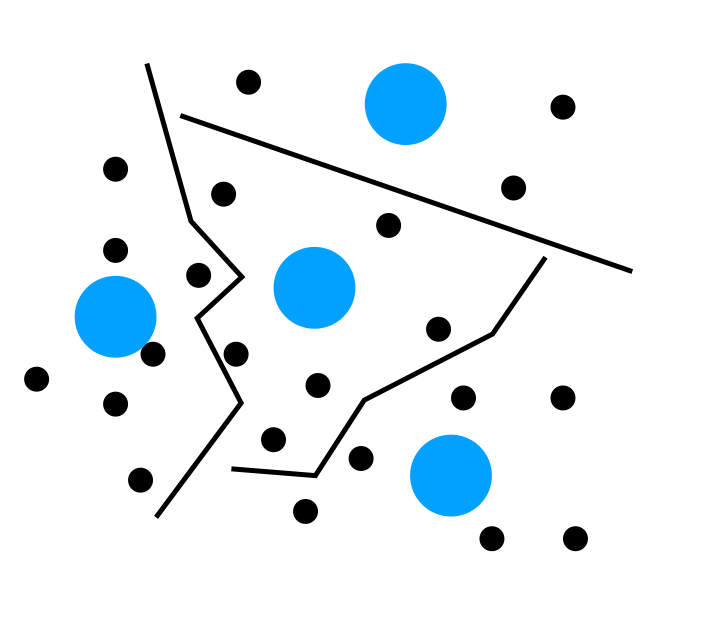
\includegraphics[width=1\linewidth]{13/4}} \\ шаг 4
\end{minipage}
\end{figure} 

После работы алгоритма, точки, находящиеся вблизи соответствующего кластера, объединяем в группы.
\end{itemize}

\subsubsection {Ранжирование}
Зачастую на запрос пользователя подходит несколько документов. Набор подходящих документов будем называть коллекцией. Как выбрать один, наиболее подходящий? Для этого считают функцию ранжирования: $R = S A$.
\begin{itemize}
\item $S$ - функция соответствия запросу. Как обсуждалось выше это может быть косинус угла между текстом и запросом или, например, \href{https://clck.ru/pvLYk}{BM25}, которая определяется следующим образом: Пусть запрос $Q$ состоит из слов $q_1, q_2, \dots q_n$ тогда $$ s = \sum_{i = 1}^n idf (q_i)
 \frac {f(q_i, D)(k_1 + 1)}{f(q_i, D) + k_1 \times \left(1 - b + b \frac{|D|}{avgdl} \right)} $$ где $n$ - количество слов в запросе, $idf(q_i)$ - idf слова $q_i$, $f(q_i, T)$ - частота слова $q_i$ в тексте $D$, $|D|$ - количество слов (мощность) текста $D$, avgdl - средняя длина слова в коллекции документов, $k_1 = 2.0, b = 0.75$;
\item A - функция авторитетности конкретного документа (эта функция своя для каждого документа и ее значение не зависит от запроса). Приведем пример определения авторитетности: Пусть есть ссылочный граф, т.е. в вершинах графа тексты, и если текст A ссылается на текст B, то в графе есть соответствующее ребро. Запустим в граф робота, который будет ходить по графу по следующему правилу: с вероятность p робот переходит из вершины, в которой находится, в одну из вершин, на которую ссылается данная, и с вероятность (1 - р) - переходит в случайную вершину графа. Чем больше раз робот прошел через вершину, тем больше ее авторитетность.
\end {itemize}



